\section*{Appendices}
\addcontentsline{toc}{section}{Appendices}
\appendix
\renewcommand\thesubsection{\Alph{subsection}}
\setcounter{subsection}{0}
\counterwithout{figure}{section}
\counterwithin{figure}{subsection}
\counterwithout{table}{section}
\counterwithin{table}{subsection}
\setupappendixheaders

\thispagestyle{plain}
\subsection{Final Dataset}
\label{apdx:final-dataset}

All variables are numeric.

\begin{xltabular}{\textwidth}{lX}
    \cline{1-2}
    \textbf{Variable Name}                               & \textbf{Curve Name in Energy Quantified API}                    \\ \cline{1-2}
    \endfirsthead

    \cline{1-2}
    \textbf{Variable Name}                               & \textbf{Curve Name in Energy Quantified API}                    \\ \cline{1-2}
    \endhead

    eq\_operational\_carbon\_emission\_t                 & DK1 Carbon Operational Emission Power Production kgCO2eq 15min Synthetic \\
    eq\_temperature                                      & DK1 Consumption Temperature °C 15min Synthetic                           \\
    eq\_dk1\_exchange\_day\_ahead\_schedule\_net\_export & DK1 Exchange Day-Ahead Schedule Net Export MWh/h H Backcast              \\
    eq\_price\_spot\_day\_ahead\_eur                     & DK1 Price Spot Day-Ahead EUR/MWh H Backcast                              \\
    eq\_residual\_power\_production\_day\_ahead          & DK1 Residual Production Day-Ahead MWh/h H Backcast                       \\
    eq\_wind\_power\_production\_onshore                 & DK1 Wind Power Production Onshore MWh/h 15min Backcast                   \\
    eq\_wind\_power\_production\_offshore                & DK1 Wind Power Production Offshore MWh/h 15min Backcast                  \\
    eq\_solar\_photovoltaic\_production                  & DK1 Solar Photovoltaic Production MWh/h 15min Backcast                   \\
    eq\_consumption                                      & DK1 Consumption MWh/h 15min Backcast                                     \\
    t\_year\_month                                       & N/A                                                                      \\
    t\_year                                              & N/A                                                                      \\
    t\_quarter\_cos                                      & N/A                                                                      \\
    t\_quarter\_sin                                      & N/A                                                                      \\
    t\_month\_cos                                        & N/A                                                                      \\
    t\_month\_sin                                        & N/A                                                                      \\
    t\_day\_cos                                          & N/A                                                                      \\
    t\_day\_sin                                          & N/A                                                                      \\
    t\_hour\_cos                                         & N/A                                                                      \\
    t\_hour\_sin                                         & N/A                                                                      \\
    t\_weeks\_since\_start                               & N/A                                                                      \\
    t\_days\_since\_start                                & N/A                                                                      \\
    t\_hours\_since\_start                               & N/A                                                                      \\ \cline{1-2}
\end{xltabular}

\clearpage

\thispagestyle{plain}
\subsection{Code Overview}
\label{apdx:code-overview}

This thesis includes all associated source code as supplementary material in the accompanying \texttt{code.zip} file. This appendix provides a little technical context for readers interested in implementation details. It assumes familiarity with Python programming and general software development concepts. The codebase is structured as a Python 3.12 library with dependencies managed through \texttt{pyproject.toml}, which specifies all required packages including TensorFlow, Polars, and other analytical libraries. The repository structure is organized as follows:

\begin{verbatim}
.
|-- src/
|   |-- analysis/
|       |-- data/
|       |   |-- bronze/             # Raw data ingestion
|       |   |   |-- eds.py
|       |   |   |-- eq.py
|       |   |-- silver/             # Data cleaning and validation
|       |   |   |-- eds.py
|       |   |   |-- eq.py
|       |   |-- gold/               # Modeling-ready datasets
|       |       |-- eds.py
|       |       |-- eq.py
|       |       |-- forecasting.py
|       |       |-- full.py
|       |-- modeling/
|           |-- main.ipynb          # Model implementation and results
|-- pyproject.toml                  # Project configuration and dependencies
\end{verbatim}
\vspace{0.2cm}

\textbf{Data Architecture:} The data processing follows a medallion architecture pattern, organizing data transformation into three distinct layers. The bronze layer contains raw data exactly as received from external sources, the silver layer applies cleaning and standardization procedures, and the gold layer produces analysis-ready datasets optimized for machine learning workflows.

\textbf{Data Sources:} The pipeline integrates two primary data sources with distinct access patterns. Files named \texttt{eds.py} handle data from Energi Data Service (publicly accessible), while \texttt{eq.py} files manage Energy Quantified data (proprietary, requiring API authentication).

\textbf{Modeling Pipeline:} The \texttt{forecasting.py} module generates the final dataset used for modeling, while \texttt{full.py} serves as the orchestration script that executes all ETL processes in the correct sequence to produce the complete dataset. The \texttt{main.ipynb} Jupyter notebook contains the complete modeling workflow, including implementation of baseline persistence models, ARIMAs, and LSTMs. The notebook is preserved with all execution outputs to provide full traceability of results.

\textbf{Note:} Data files (.parquet) are excluded from the submission due to size constraints and proprietary licensing restrictions. The ETL pipeline can regenerate all datasets when provided with appropriate API keys.

\clearpage

\thispagestyle{plain}
\subsection{LSTMs Predictions vs Actuals}
\label{apdx:lstms-predictions-vs-actuals}

\begin{figure}[ht]
    \centering
    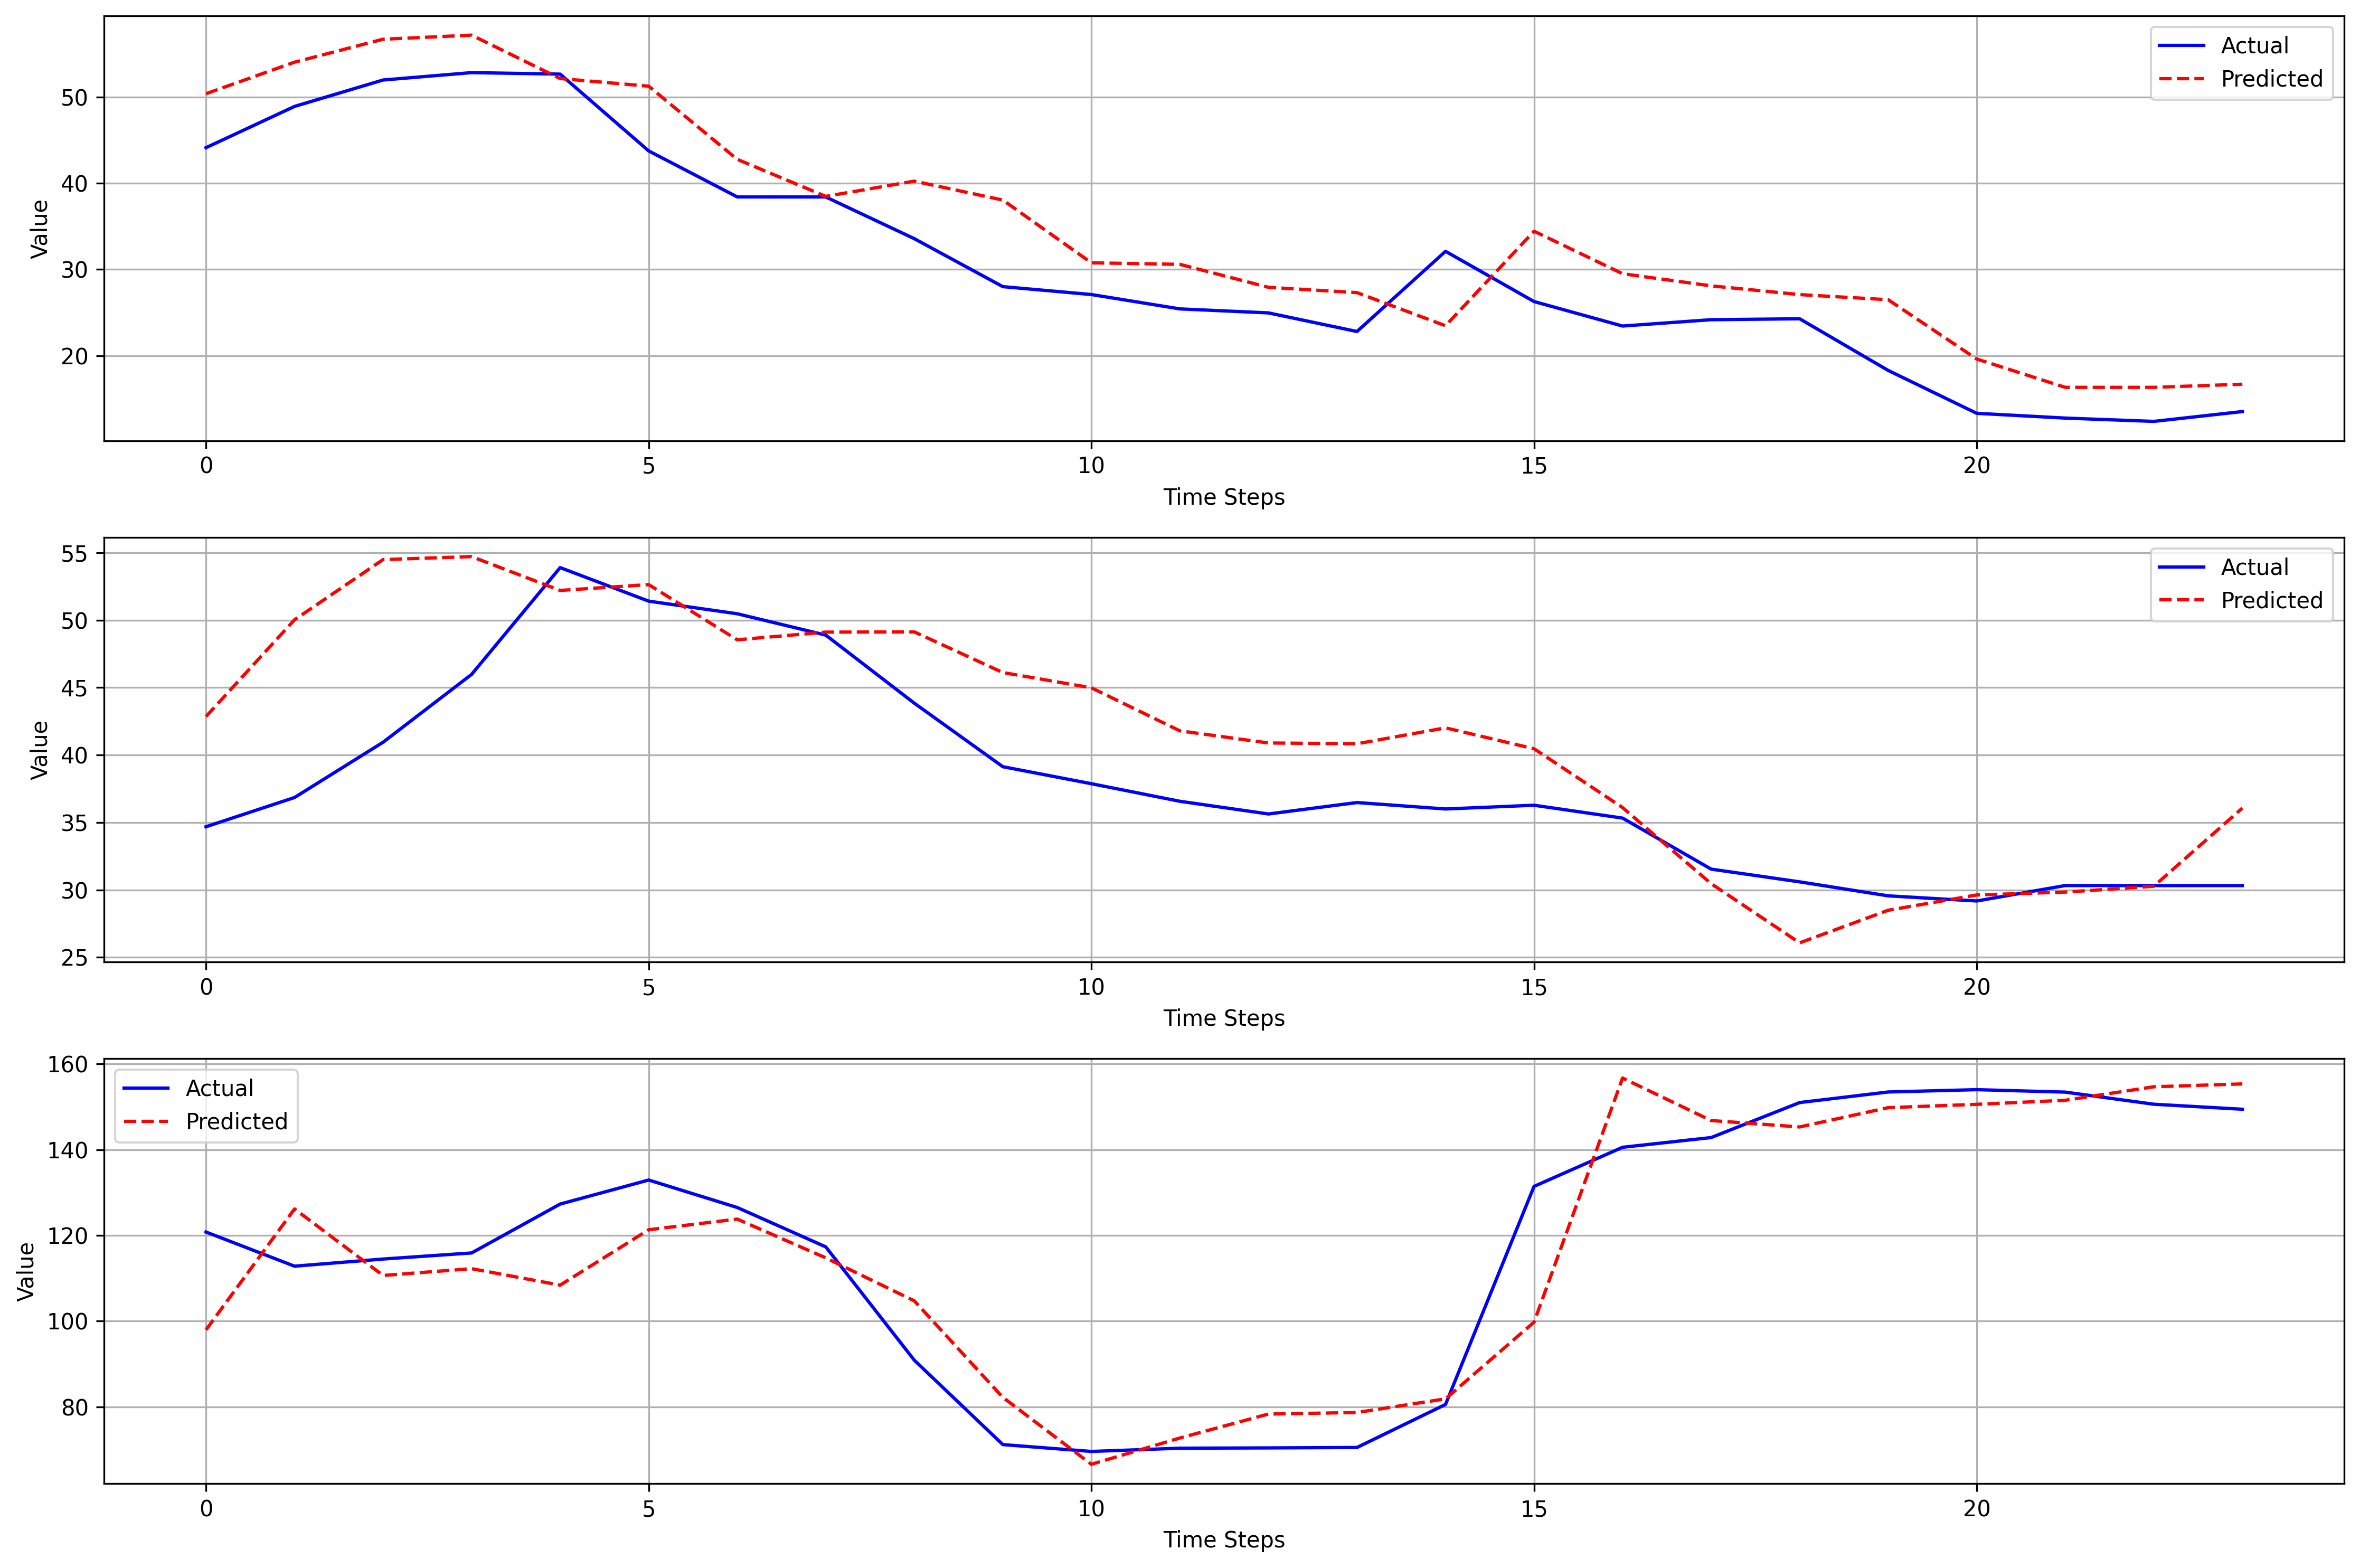
\includegraphics[width=16cm]{sections/figures/lstm_point_test_pred_vs_acts.png}
    \caption{LSTM 1-hour Model Predictions vs Actuals (Three random drawn samples)}
    \label{fig:lstm-point-test-pred-vs-acts}
\end{figure}

\begin{figure}[ht]
    \centering
    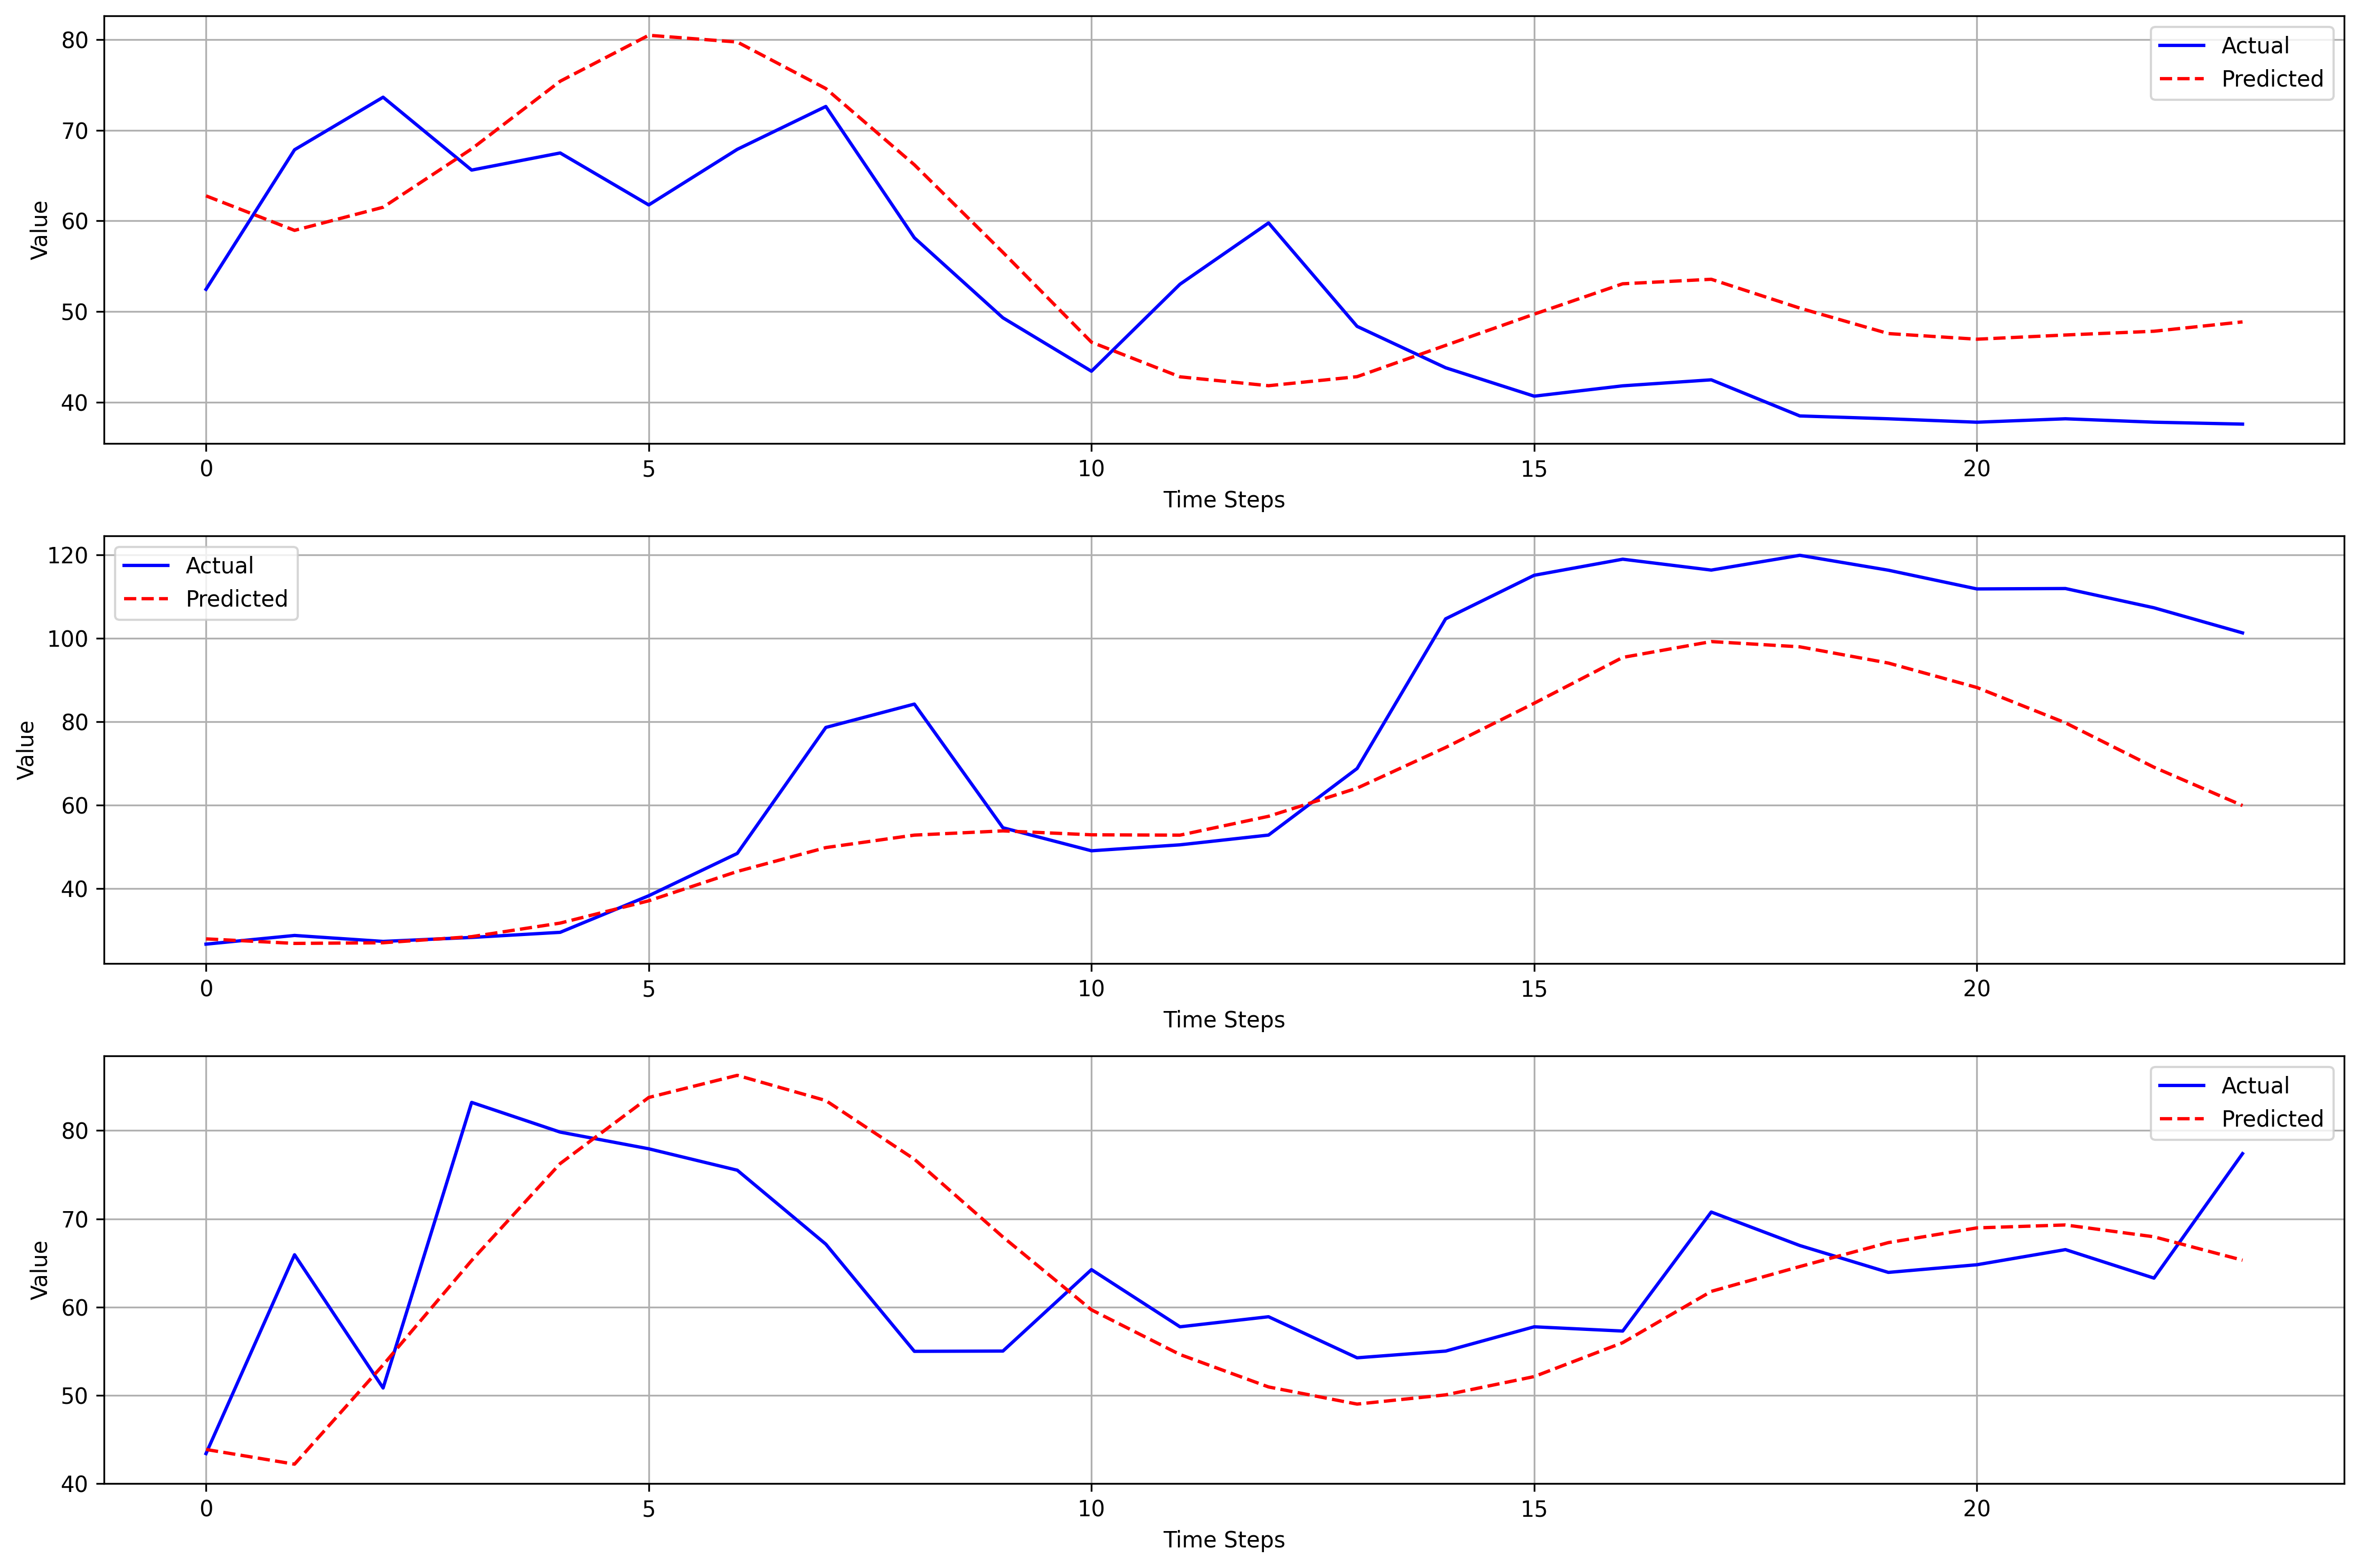
\includegraphics[width=16cm]{sections/figures/lstm_seq_test_pred_vs_acts.png}
    \caption{LSTM 24-hour Model Predictions vs Actuals (Three random drawn samples)}
    \label{fig:lstm-seq-test-pred-vs-acts}
\end{figure}

\clearpage

\thispagestyle{plain}
\subsection{Comprehensive Model Error Metrics}
\label{apdx:comprehensive-model-error-metrics}

\begin{table}[ht]
    \centering
    \begin{tabular}{lccc}
        \hline
        \textbf{Model}                   & \textbf{Train MAE\phantom{0}} & \textbf{Validation MAE\phantom{0}} & \textbf{Test MAE\phantom{0}} \\ \hline
        Naive persistence model, 1-hour  & \phantom{0}8.25               & \phantom{0}6.63                    & \phantom{0}6.13              \\
        ARIMA(5,0,5), 1-hour             & \phantom{0}7.90               & \phantom{0}6.35                    & \phantom{0}5.99              \\
        Single-Layer LSTM, 1-hour        & \phantom{0}7.10               & \phantom{0}6.08                    & \phantom{0}6.28              \\
        Naive persistence model, 24-hour & 24.89                         & 18.19                              & 20.33                        \\
        ARIMA(5,0,5), 24-hour            & 22.04                         & 15.46                              & 18.21                        \\
        Encoder-Decoder LSTM, 24-hour    & 14.08                         & 16.61                              & 16.32                        \\ \hline
    \end{tabular}
    \caption{Overview of MAEs in tonnes \cotwoe{} across all models}
    \label{tab:overview-maes-across-models}
\end{table}

\vspace{1cm}

\begin{table}[ht]
    \centering
    \begin{tabular}{lccc}
        \hline
        \textbf{Model}                   & \textbf{Train RMSE} & \textbf{Validation RMSE} & \textbf{Test RMSE} \\ \hline
        Naive persistence Model, 1-hour  & 13.15               & 10.83                    & 10.54              \\
        ARIMA(5,0,5), 1-hour             & 12.09               & \phantom{0}9.52          & \phantom{0}9.43    \\
        Single-Layer LSTM, 1-hour        & 10.60               & \phantom{0}8.59          & \phantom{0}9.01    \\
        Naive persistence model, 24-hour & 38.43               & 26.86                    & 29.75              \\
        ARIMA(5,0,5), 24-hour            & 33.18               & 21.58                    & 25.03              \\
        Encoder-Decoder LSTM, 24-hour    & 19.90               & 21.51                    & 22.20              \\ \hline
    \end{tabular}
    \caption{Overview of RMSEs in tonnes \cotwoe{} across all models}
    \label{tab:overview-rmse-across-models}
\end{table}

\clearpage

\thispagestyle{plain}
\subsection{Full Feature Importance Analysis Results}
\label{apdx:full-feature-importance-analysis-results}

\begin{xltabular}{\textwidth}{Xc}
    \hline
    \textbf{Feature}                                             & \textbf{Importance} \\ \hline
    \endfirsthead

    \hline
    \textbf{Feature}                                             & \textbf{Importance} \\ \hline
    \endhead

    \hline
    \multicolumn{2}{r}{\textit{Table continued on next page...}} \\
    \endfoot

    \endlastfoot

    hist\_eq\_operational\_carbon\_emission\_t                   & 22.58               \\
    future\_eq\_solar\_photovoltaic\_production                  & 4.94                \\
    future\_eq\_temperature                                      & 3.67                \\
    future\_t\_hour\_cos                                         & 2.82                \\
    future\_eq\_consumption                                      & 2.19                \\
    hist\_eq\_wind\_power\_production\_offshore                  & 1.38                \\
    hist\_eq\_solar\_photovoltaic\_production                    & 1.36                \\
    future\_t\_quarter\_cos                                      & 1.36                \\
    future\_eq\_residual\_power\_production\_day\_ahead          & 0.93                \\
    future\_t\_quarter\_sin                                      & 0.81                \\
    future\_eq\_price\_spot\_day\_ahead\_eur                     & 0.65                \\
    hist\_t\_day\_cos                                            & 0.64                \\
    hist\_t\_month\_cos                                          & -0.44               \\
    hist\_t\_month\_sin                                          & -0.43               \\
    hist\_t\_hours\_since\_start                                 & 0.42                \\
    hist\_t\_quarter\_sin                                        & -0.38               \\
    hist\_t\_hour\_cos                                           & 0.36                \\
    future\_t\_month\_sin                                        & -0.33               \\
    future\_t\_day\_cos                                          & 0.31                \\
    future\_t\_day\_sin                                          & 0.30                \\
    future\_t\_year\_month                                       & 0.29                \\
    future\_t\_hour\_sin                                         & 0.26                \\
    hist\_eq\_wind\_power\_production\_onshore                   & 0.21                \\
    hist\_t\_days\_since\_start                                  & -0.21               \\
    hist\_eq\_temperature                                        & 0.14                \\
    hist\_t\_day\_sin                                            & 0.13                \\
    future\_t\_month\_cos                                        & 0.13                \\
    hist\_t\_weeks\_since\_start                                 & -0.12               \\
    future\_eq\_wind\_power\_production\_onshore                 & -0.10               \\
    future\_t\_weeks\_since\_start                               & -0.06               \\
    hist\_t\_hour\_sin                                           & 0.06                \\
    hist\_t\_year\_month                                         & 0.05                \\
    future\_t\_days\_since\_start                                & -0.05               \\
    hist\_eq\_residual\_power\_production\_day\_ahead            & 0.03                \\
    future\_t\_hours\_since\_start                               & -0.03               \\
    future\_eq\_dk1\_exchange\_day\_ahead\_schedule\_net\_export & -0.02               \\
    hist\_eq\_dk1\_exchange\_day\_ahead\_schedule\_net\_export   & -0.02               \\
    hist\_eq\_consumption                                        & 0.02                \\
    hist\_eq\_price\_spot\_day\_ahead\_eur                       & 0.02                \\
    hist\_t\_quarter\_cos                                        & 0.01                \\
    future\_eq\_wind\_power\_production\_offshore                & -0.01               \\
    hist\_t\_year                                                & 0.00                \\
    future\_t\_year                                              & 0.00                \\ \hline
    \caption{Feature Importance Analysis RMSE in tonnes \cotwoe{}}
    \label{tab:feature-importance-analysis-rmse}
\end{xltabular}

\clearpage

\thispagestyle{plain}
\subsection{Manufacturing Impact Analysis: Assumptions and Detailed Calculations}
\label{apdx:manufacturing-impact-analysis}

Besides the assumptions stated in \autoref{subsec:practical-impact-for-manufacturing-companies}, the calculations also rely on several key underlying assumptions: 1) manufacturing facilities possess sufficient operational flexibility to shift 25\% of energy-intensive processes based on carbon forecasting without significant productivity losses, 2) the DK1 grid maintains adequate variability in carbon emissions to make demand response scheduling meaningful, 3) companies actively respond to emission forecasting information with economic incentives beyond electricity pricing, 4) forecasting accuracy improvements translate proportionally to real-world scheduling benefits, and 5) implementation costs for demand response infrastructure are excluded from the economic analysis. While these assumptions represent simplifications of complex industrial operations, they provide a reasonable foundation for estimating the potential magnitude of benefits from improved carbon emission forecasting.

\begin{xltabular}{\textwidth}{lX}
    \hline
    \textbf{Derived Value}              & \textbf{Calculation} \\ \hline
    \endfirsthead

    5.7\% improvement (vs ARIMA)            & \(11.3\% \div 2\)                                                                                    \\
    12.7\% improvement (vs naive)           & \(25.4\% \div 2\)                                                                                    \\
    855 tonnes \cotwoe{} reduction          & \(50 \text{ GWh} \times 300 \text{ kg \cotwoe{}/MWh} \times 5.7\%\)                                  \\
    1,905 tonnes \cotwoe{} reduction        & \(50 \text{ GWh} \times 300 \text{ kg \cotwoe{}/MWh} \times 12.7\%\)                                 \\
    \euro72,700 cost savings                    & \(855 \text{ tonnes} \times \text{\euro}85/\text{tonne}\)                                                \\
    \euro161,900 cost savings                   & \(1,905 \text{ tonnes} \times \text{\euro}85/\text{tonne}\)                                              \\
    20 annual TWh and 37.5\% industry share & Based on the dataset \texttt{PrivIndustryConsumptionMunicipalityMonth} form \textcite{energidataservice2025}. \\
    1.875 TWh industrial consumption        & \(20 \text{ TWh} \times 37.5\% \times 25\%\)                                                         \\
    32,063 tonnes \cotwoe{} (grid-wide)     & \(1.875 \text{ TWh} \times 300 \text{ kg \cotwoe{}/MWh} \times 5.7\%\)                               \\
    71,438 tonnes \cotwoe{} (grid-wide)     & \(1.875 \text{ TWh} \times 300 \text{ kg \cotwoe{}/MWh} \times 12.7\%\)                              \\
    \euro2.7 million economic value             & \(32,063 \text{ tonnes} \times \text{\euro}85/\text{tonne}\)                                             \\
    \euro6.1 million economic value             & \(71,438 \text{ tonnes} \times \text{\euro}85/\text{tonne}\)                                             \\
    6,970 vehicles equivalent               & \(32,063 \text{ tonnes} \div 4.6 \text{ tonnes per vehicle/year}\)                                   \\
    15,530 vehicles equivalent              & \(71,438 \text{ tonnes} \div 4.6 \text{ tonnes per vehicle/year}\)                                   \\

    \hline
    \caption{Calculation Details for Manufacturing Impact Analysis}
    \label{tab:manufacturing-impact-calculations}
\end{xltabular}

\clearpage

\thispagestyle{plain}
\subsection{Energinet Impact Analysis: Assumptions and Detailed Calculations}
\label{apdx:energinet-impact-analysis}

Besides the assumptions stated in \autoref{subsec:practical-impact-for-energinet}, the calculations also rely on several key underlying assumptions: 1) Energinet possesses sufficient operational flexibility to implement proactive grid management strategies based on carbon forecasting without compromising grid security, 2) the DK1 grid maintains adequate mFRR activation frequency to make demand response coordination and cross-border scheduling optimization meaningful, 3) transmission system operators actively utilize emission forecasting information for operational decision-making beyond current practices, 4) forecasting accuracy improvements translate to operational benefits at a reduced rate (25\%) compared to manufacturing due to real-time constraints and regulatory requirements, and 5) implementation costs for enhanced forecasting infrastructure integration are excluded from the economic analysis. While these assumptions represent simplifications of complex transmission system operations, they provide a reasonable foundation for estimating the potential magnitude of benefits from improved carbon emission forecasting for TSO operations.

\begin{xltabular}{\textwidth}{lX}
    \hline
    \textbf{Derived Value}              & \textbf{Calculation} \\ \hline
    \endfirsthead

    2.8\% improvement (vs ARIMA)                 & \(11.3\% \times 25\%\)                                                                                                                                                       \\
    6.4\% improvement (vs naive)                 & \(25.4\% \times 25\%\)                                                                                                                                                       \\
    17 GWh avoided mFRR (vs ARIMA)               & \(0.6 \text{ TWh} \times 2.8\%\)                                                                                                                                             \\
    38 GWh avoided mFRR (vs naive)               & \(0.6 \text{ TWh} \times 6.4\%\)                                                                                                                                             \\
    8,500 tonnes \cotwoe{} reduction (vs ARIMA)  & \(17 \text{ GWh} \times 1000 \text{ MWh/GWh} \times 500 \text{ kg \cotwoe{}/MWh} \div 1000\)                                                                                 \\
    19,000 tonnes \cotwoe{} reduction (vs naive) & \(38 \text{ GWh} \times 1000 \text{ MWh/GWh} \times 500 \text{ kg \cotwoe{}/MWh} \div 1000\)                                                                                 \\
    0.6 TWh annual mFRR baseline                 & Based on Energi Data Service API dataset \texttt{RegulatingBalancePowerdata}, averaging 2021-2023 data: (550,115 + 612,067 + 603,756 MWh) = 589k MWh, approximately 0.6 TWh. \\
    500 kg \cotwoe{}/MWh emission factor         & Based on Energi Data Service API dataset \texttt{CO2Emis}, representing 3-year mean for DK1 hours when mFRR-up was activated, reflecting the marginal fossil stack.          \\
    \euro3.2 million cost savings (vs ARIMA)         & \(17 \text{ GWh} \times 1000 \text{ MWh/GWh} \times \text{\euro}186/\text{MWh} \div 1,000,000\)                                                                                  \\
    \euro7.1 million cost savings (vs naive)         & \(38 \text{ GWh} \times 1000 \text{ MWh/GWh} \times \text{\euro}186/\text{MWh} \div 1,000,000\)                                                                                  \\
    1,850 vehicles equivalent (vs ARIMA)         & \(8,500 \text{ tonnes} \div 4.6 \text{ tonnes per vehicle/year}\)                                                                                                            \\
    4,100 vehicles equivalent (vs naive)         & \(19,000 \text{ tonnes} \div 4.6 \text{ tonnes per vehicle/year}\)                                                                                                           \\

    \hline
    \caption{Calculation Details for Energinet Impact Analysis}
    \label{tab:energinet-impact-calculations}
\end{xltabular}

\clearpage
